Ud fra sprint 1 har vi erfaret at for store user stories giver en uklar pr�sentation af fremskridt p� vores burndown. Vi startede s�ledes sprint 2 med at dele nogle af vores user stories op. Herefter lavede vi planning poker for at f� et mere n�jagtigt estimat af hvor lang tid de forskellige stories ville tage. Endvidere, for samtidigt at f� et mere n�jagtigt burndown, begyndte vi at br�nde det ned i mandetimer fremfor user stories, samt s�tte mandetimer p� de enkelte tasks.
Sprintet 2 handlede i h�j grad om at lave user stories for database samt koblingen mellem databasen og foodmap.

\subsection{Velocity}
Vi har ikke �ndret p� vores velocity fra sprint 1, da vi mener at vi ikke fik br�ndt ned p� burndown pga. for store user stories og d�rlig estimering. Vi forventede derfor at have 4 mandetimer om dagen per mand i gruppen. Dvs. 8 mandetimer om dagen med 2 hold med 4 arbejdsdage. \\
Story points og mandetimer forblev det samme som i sprint 1: 5 story points pr 8 mandetimer, 0,625 story points per mandetime, 32 mande timer i sprintet og 20 story points per uge, dvs. 5 story points per dag.

\begin{figure}[H]
\begin{center}
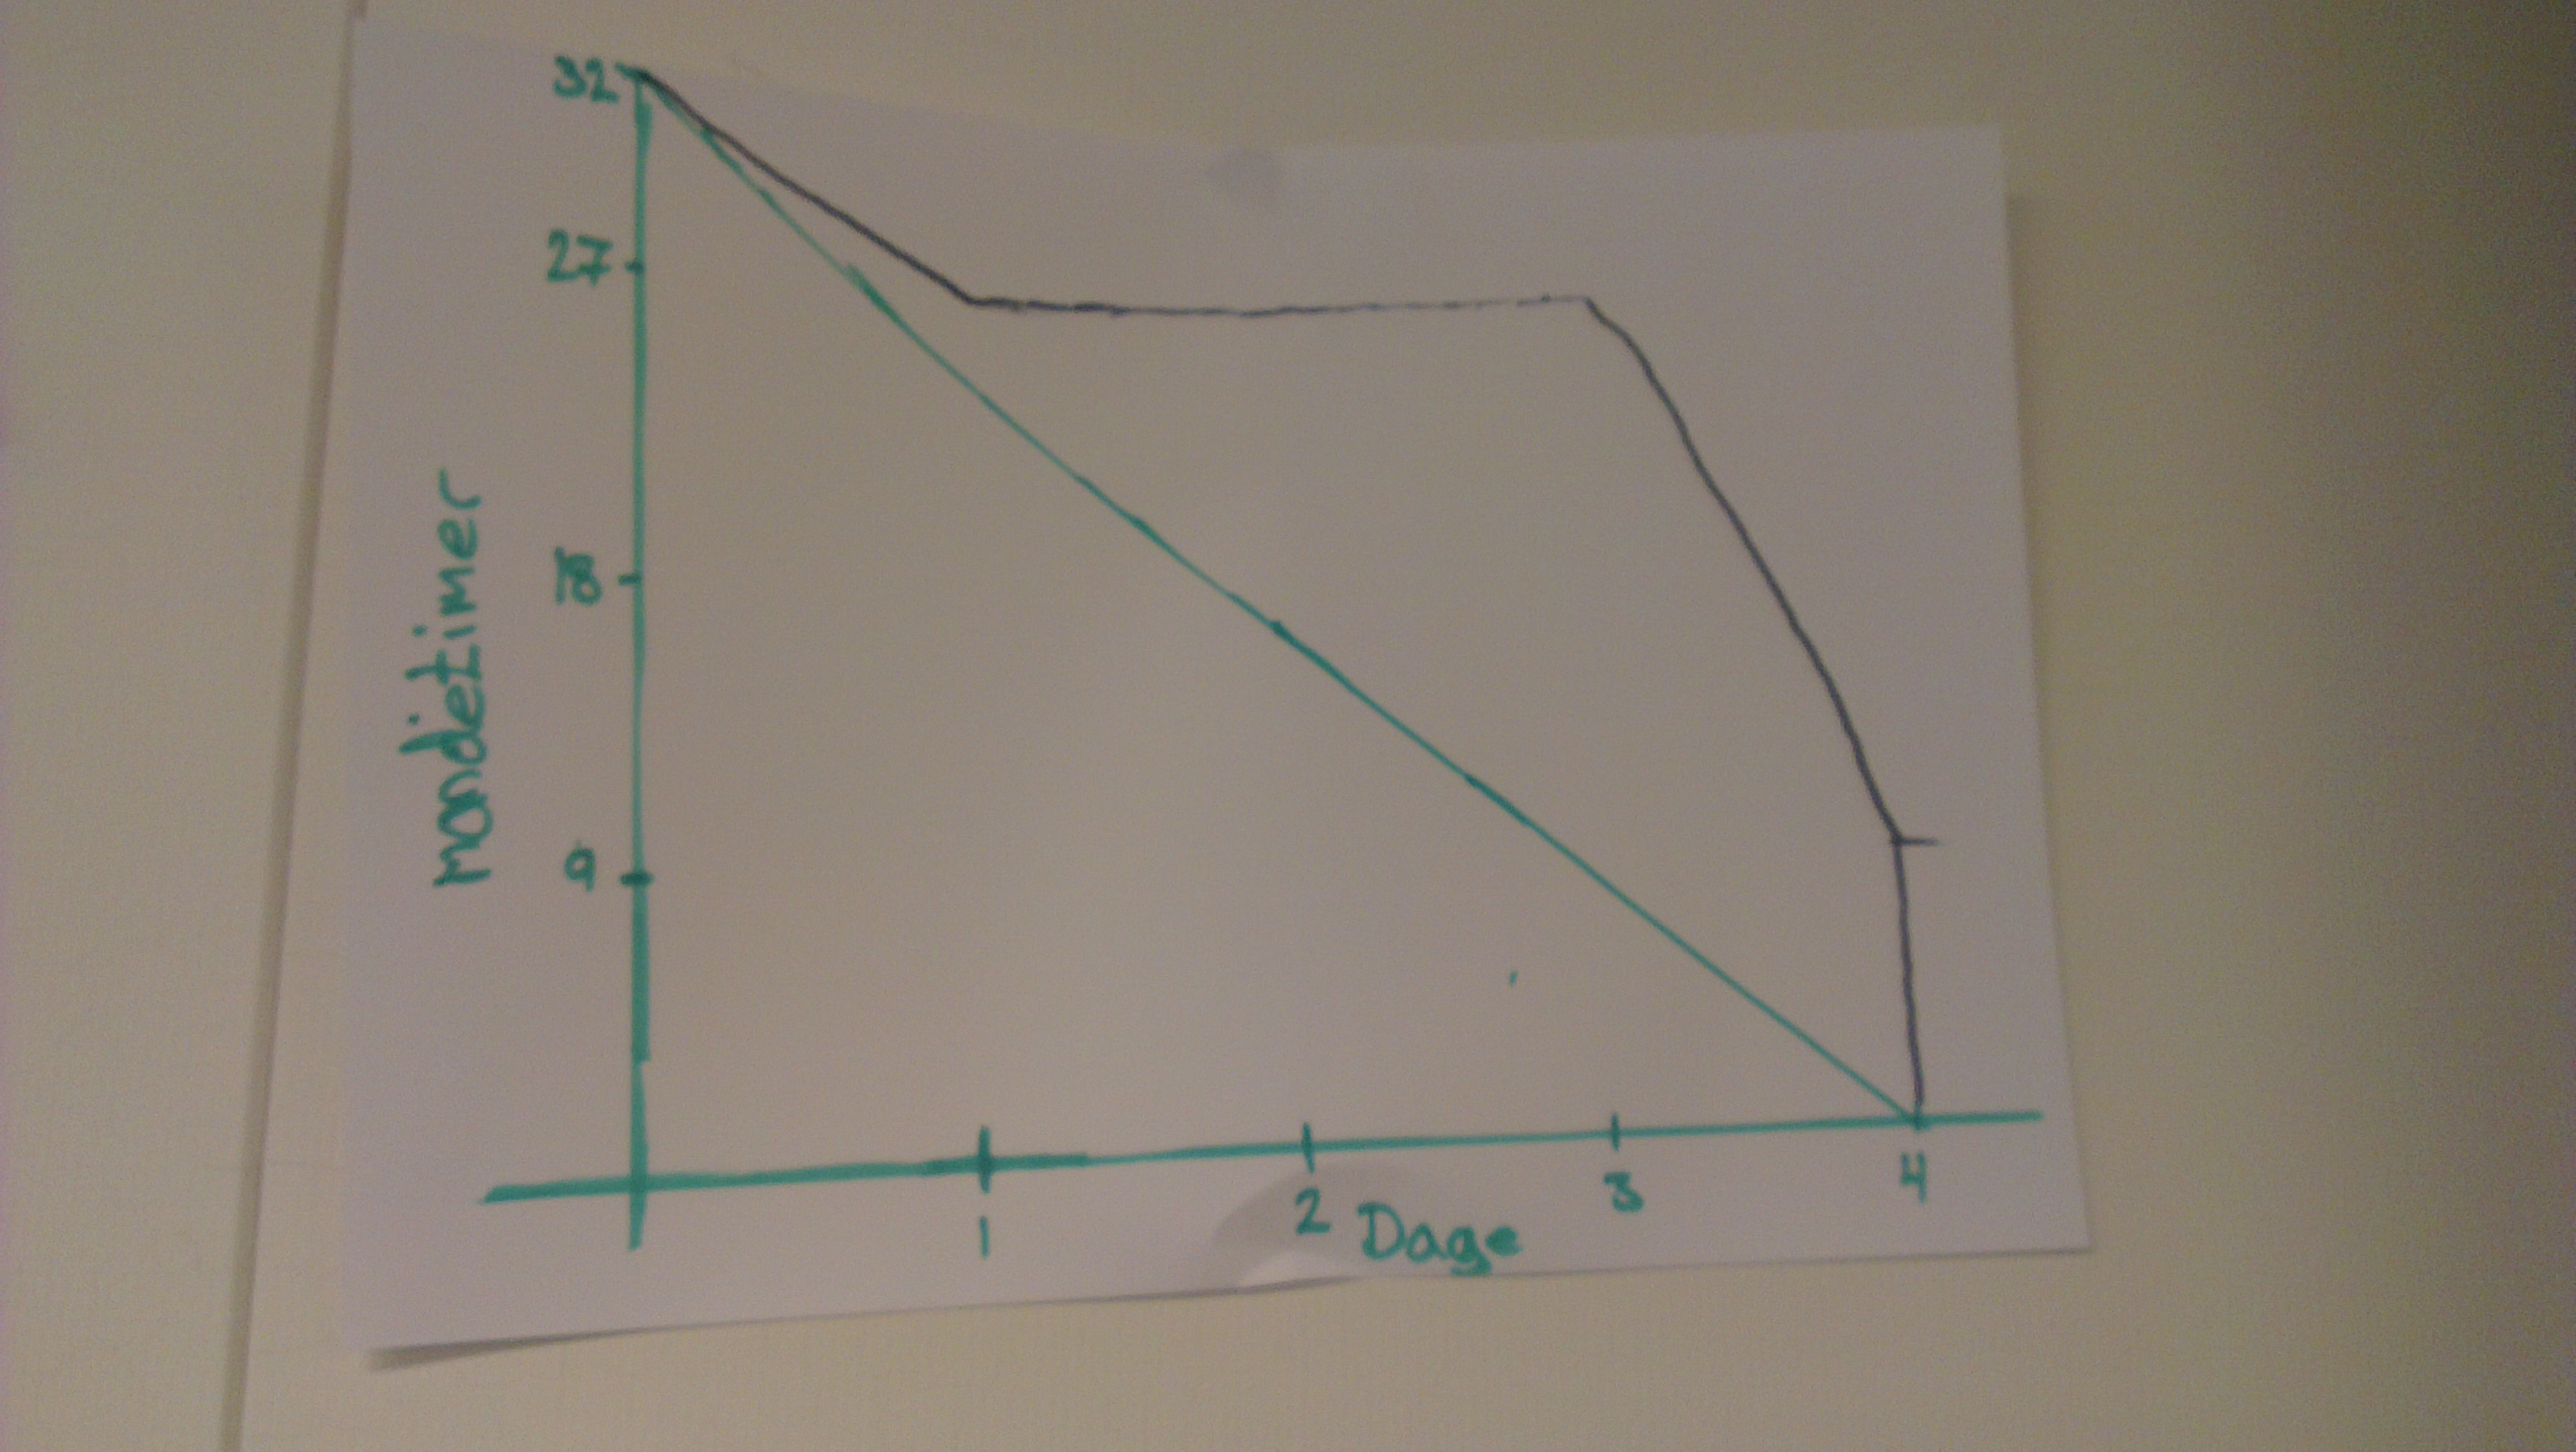
\includegraphics[scale=0.10]{includes/billeder/sprint2.jpg}
\caption{Sprint 2 burndown}
\label{fig:sprint2:burndown}
\end{center}
\end{figure}

\subsection{Produkt backlog}
Backlog lavet den 9.12.2013 i starten af sprint 2. \\
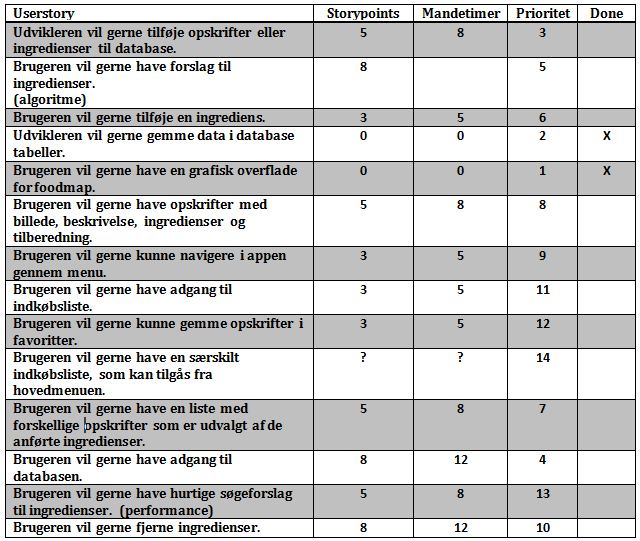
\includegraphics[scale=0.60]{includes/billeder/productbacklog_sprint2.png}

\subsection{Sprint backlog}
I sprint 2 fokuserede vi p� f�lgende user stories:

\begin{figure}[H]
\begin{center}
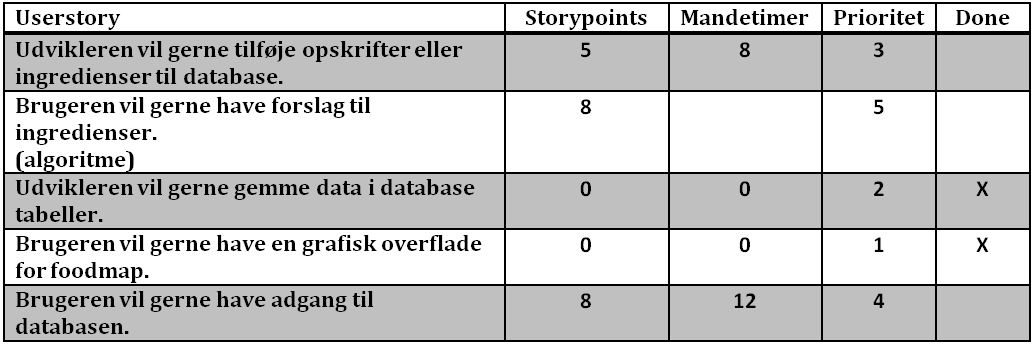
\includegraphics[scale=0.55]{includes/billeder/sprintbacklog_sprint2.png}
\caption{Sprint backlog}
\label{fig:sprint2:sprintbacklog}
\end{center}
\end{figure}

Database tabeller og basic gui satte vi til 0 mandetimer og done, da de var f�rdige efter vi opdelte dem, da de tidligere var dele af st�rre user stories. 

\subsection{Xp og scrum praktikker}
I sprint 2 benyttede vi XP praktikkerne: stand-up meeting, planning poker, par programmering, kollektivt kode ejerskab, refactoring, kodestandarder, metafor og simpelt design. \\
Vi havde en scrum master, men product owner droppede vi, da det ikke giver s� meget mening i en gruppe af 3.

\subsection{Produkt review}
Til produkt reviewet var det planen at vi ville vise vores gui med database adgang, men Android emuleratoren fejlede og pr�sentationen faldt derfor til bunden. Det endte med at vi kun viste selve databasen med data. 

\subsection{Retrospektive}
I sprint 2 blev vi endeligt f�rdige med b�de databasen og koblingen mellem database og gui, dog f�rst efter at have en del overarbejde. Samtidigt havde vi overvurderet hvor mange ressourcer vi egentligt havde til r�dighed og n�ede derfor at br�nde 20 ud af 32 mandetimer.

\subsubsection*{Hvad gik godt}
Sprint 2 gik meget bedre end sprint 1 idet at vi endeligt fik styr p� database delen af vores projekt, dog efter meget overarbejde. Samtidigt fik vi en positiv oplevelse af at f� opsplittet vores user stories bedre, da de dermed blev mere pr�cise b�de i formulering og estimering. 

\subsubsection*{Hvad gik mindre godt}
Vi skulle have v�ret lidt bedre forberedt til produkt reviewet; det kunne m�ske have v�ret muligt at undg� problemer med emulatoren og kunden havde f�et et bedre indtryk af hvad vi havde lavet.

\subsubsection*{Hvad �ndrer vi til n�ste sprint}
En revurdering af vores velocity, da vi �benlyst havde vurderet den for h�jt igen og m�tte s�ge at lave et mere overkommeligt m�l.